\begin{frame}[t]\vspace{-1em}
    \titlepage
\end{frame}
\note{
    Welcome to the Sonata and CHERIoT part of this workshop.
    My name is Marno van der Maas and I'm here with Douglas Reis and John Thomson from lowRISC.
}

\begin{frame}{Outline}
  \tableofcontents
\end{frame}
\note{
  This is the outline of what I'll talk about before we start the hands-on workshop.
  First I'll give a general introduction and then give you and overview of Sonata and CHERIoT.
  Finally, I'll go through what we'll do in the workshop.
}

%%%%%%%%%%%%%%%%%%%%%%
\section{Introduction}
%%%%%%%%%%%%%%%%%%%%%%

\begin{frame}
  \frametitle{Morello vs CHERIoT}
  \centering
  \begin{center}
  \begin{tabular}{r | l | l}
    & Morello & CHERIoT \\ \hline
    Use-case & Application-class & Embedded \\ \hline
    Virtual memory & Yes & No \\ \hline
    Address size & 64-bits & 32-bits \\ \hline
    Operating system & CheriBSD & CHERIoT RTOS \\ \hline
    RAM size & $>1$ GiB & $<1$ MiB \\
  \end{tabular}
  \end{center}
\end{frame}
\note{
  This morning we were focussed on Morello, how does that exercise compare to the one we will do now?
  This table shows some of the key differences.
}

\begin{frame}
    \frametitle{Why embedded?}
    \centering
    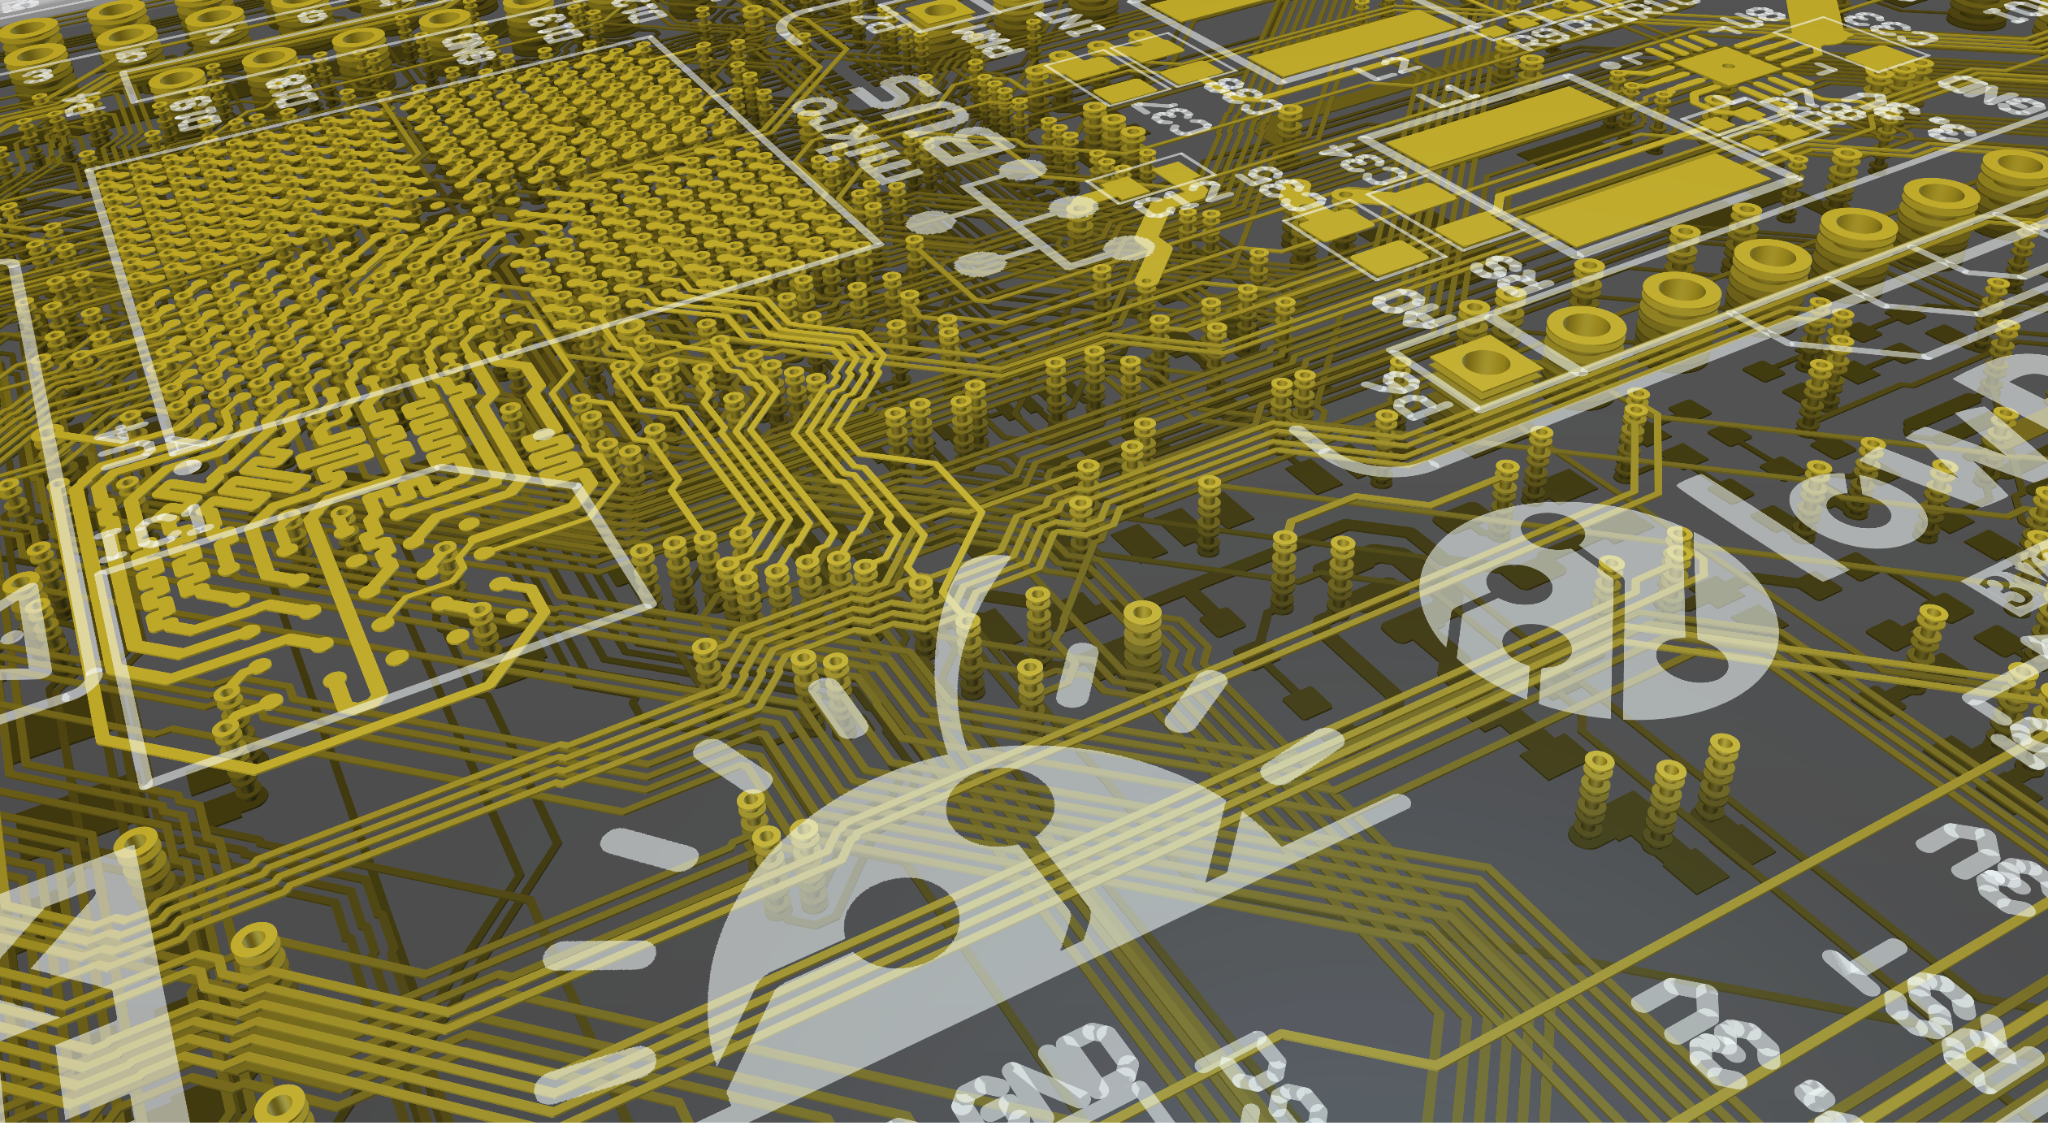
\includegraphics[height=0.8\textheight]{img/embedded.png}
\end{frame}
\note{
    A lot of the initial CHERI research was done on application class processors and proving that the technology could work with rich operating systems, third party applications, a large codebase and modern compilers.
    This was important to prove the technology.

    We believe in the step towards commercialization, embedded systems may be a better place to start because vendors usually have more control over the whole software stack and can recompile everything to use pure capability.
    Sonata provides an open source platform to make this happen.
}

%%%%%%%%%%%%%%%%%%%%%
\section{Sonata overview}
%%%%%%%%%%%%%%%%%%%%%

\begin{frame}
    \centering
    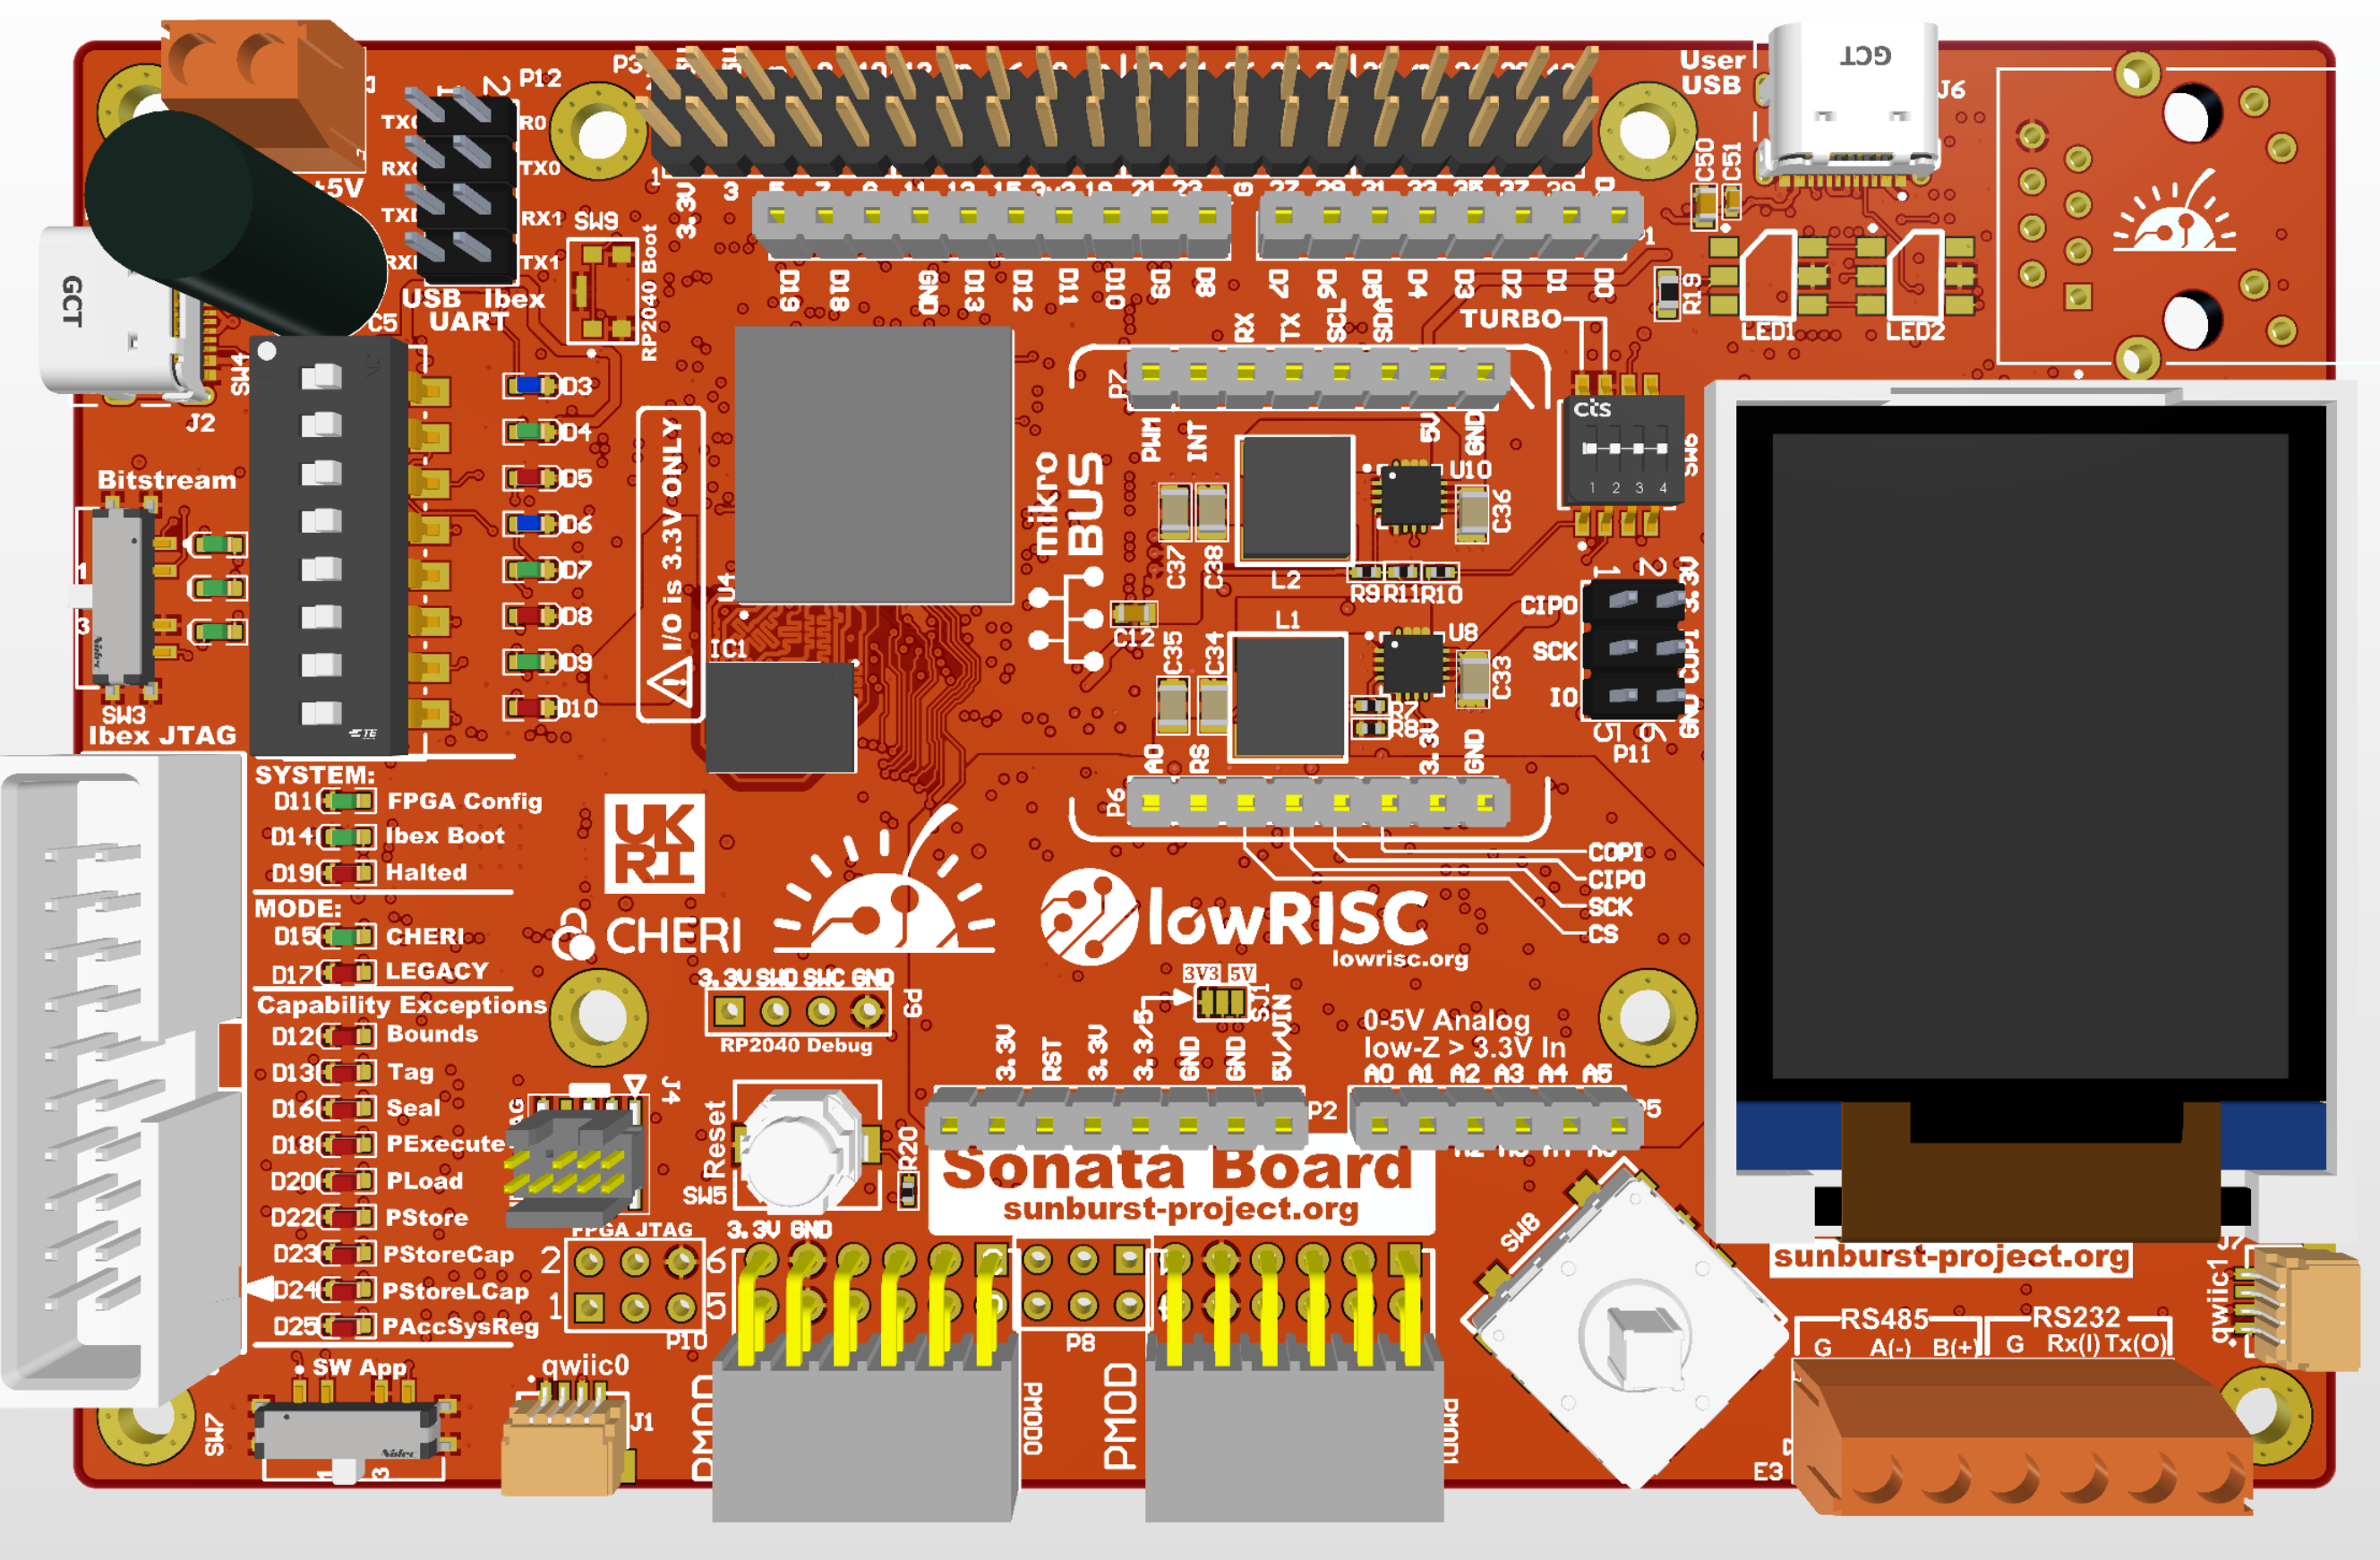
\includegraphics[width=0.9\textwidth]{img/pcb.png}
\end{frame}
\note{
    Here's a picture of the Sonata board!
    It is a fully open source platform to get CHERI hardware in the hands of embedded systems engineers.
    Sonata is easy to use, for example USB provides power, allows programming the FPGA and can be used as a serial UART terminal.
}

\begin{frame}
    \centering
    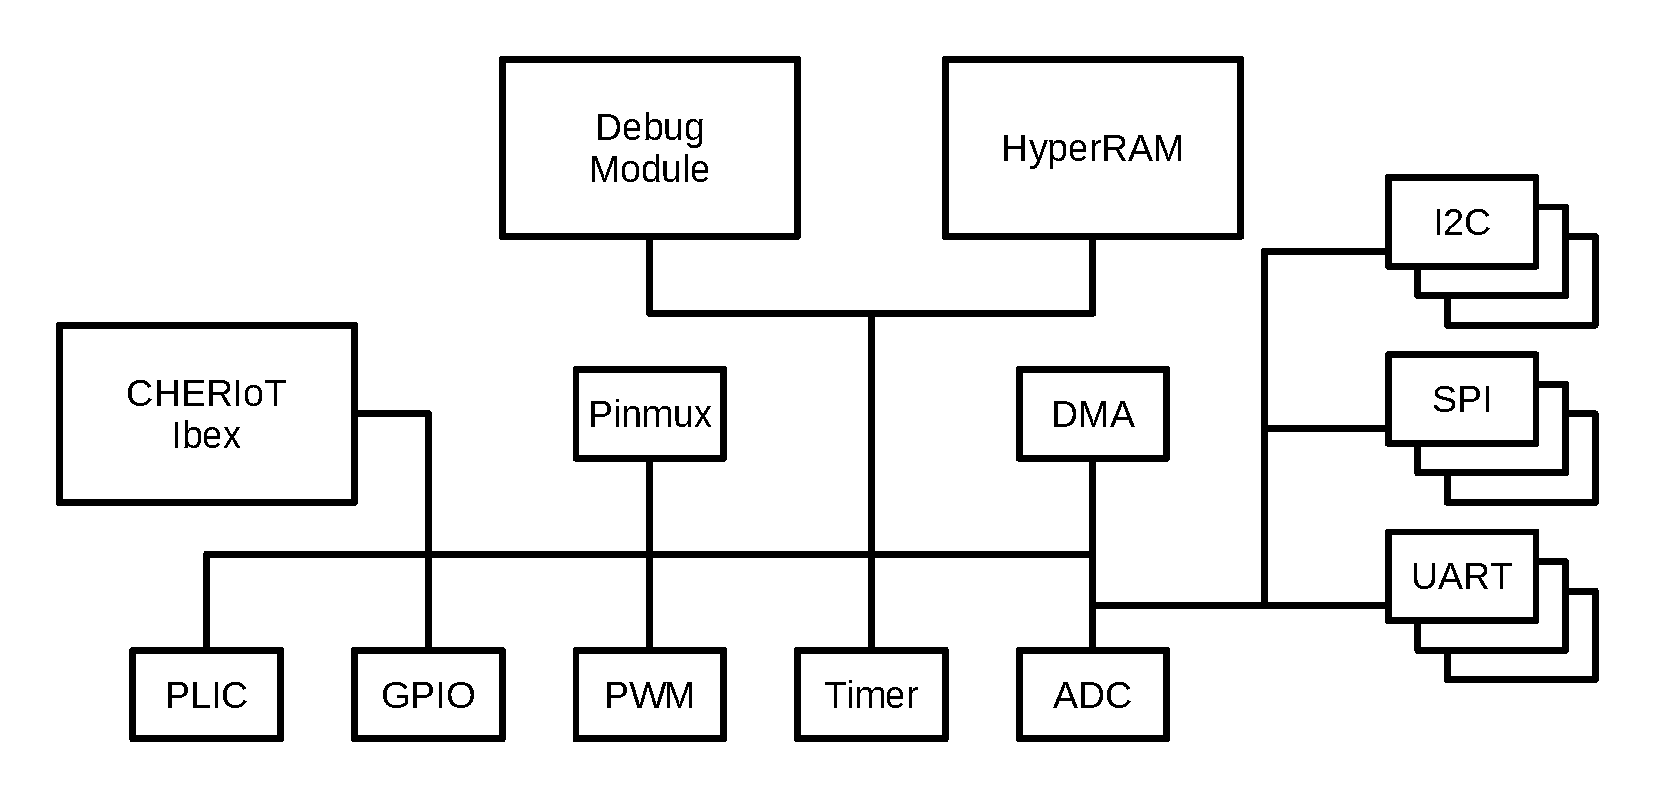
\includegraphics[width=0.9\textwidth]{img/block-diagram.pdf}
\end{frame}
\note{
    Sonata is all about being usable, debuggable, connectable, extendable and interactive.
    To achieve all of this, we need a balance of IP blocks which you can see in this block diagram.

    There is also a big focus on configurability.
    For example the pinmux can be used to drive an LED by a PWM instead of a GPIO.
    Map I2C, SPI and UART onto different headers.
}

\begin{frame}
    \frametitle{Extendable}
    \begin{itemize}
        \item Raspberry Pi Hat
        \item Arduino Shield
        \item mikroBus Click
        \item SparkFun QWIIC
        \item PMOD 0, 1 and C
        \item RS-232 RS-485
        \item USB device
    \end{itemize}
\end{frame}
\note{
    And any niche use-cases can be achieved using any of the extension headers provided.
    You can buy off the shelf boards to for example add wireless functionality.
    The hat, shield and click have connectors on the top of the board.
    QWIIC uses I2C to daisy chain boards together (two connectors on the side).
    There are two PMOD connectors on the bottom as well as RS-232 and RS-485 connectors.
}

\begin{frame}
  \frametitle{V1.0 release}
  \begin{itemize}
    \item PCB and board design
    \item Drag and drop programming using RP2040
    \item Pinmux for mapping IP blocks onto pins
    \item GPIO and PWM
    \item Bootloader with support for software slots
    \item Bitstream switching
    \item Simulator, FPGA and CI
    \item 40 MHz clock, 128 KiB SRAM, 1 MiB HyperRAM
    \item Capability memory architecture including hardware revocation
    \item Nix development environment
  \end{itemize}
\end{frame}
\note{
  For more details see: \url{https://github.com/lowRISC/sonata-system/releases/tag/v1.0}

  To buy Sonata se: \url{https://tinyurl.com/sonata-int}
}

%%%%%%%%%%%%%%%%%%%%
\section{CHERIoT overview}
%%%%%%%%%%%%%%%%%%%%

\begin{frame}
    \frametitle{Capability format}

    \begin{itemize}
        \item 32-bit address
        \item 22-bit compressed base and top
        \item 3-bit object type for sealing
        \item 6-bit compressed permissions
        \item 1-bit reserved
        \item \textbf{Total:} 64-bits
        \item 1-bit out-of-band validity
    \end{itemize}
\end{frame}
\note{
    64-bit capabilities are a lot more difficult than 128-bit ones because you only have 32-bits of meta-data.
    See the full ISA specification here: \url{https://github.com/CHERIoT-Platform/cheriot-sail/tree/main/archdoc}

    The way CHERIoT solves this is by compression of permissions and using object type indirection for sealing.
}

\begin{frame}
    \frametitle{Compartmentalization}
  \begin{itemize}
    \item CHERIoT compartments
      \begin{itemize}
        \item Program counter capability
        \item Global capability pointer
        \item Export table
        \item Import table
      \end{itemize}
    \item RTOS compartments
    \begin{itemize}
        \item Memory allocator
        \item Scheduler
        \item Revoker
    \end{itemize}
  \end{itemize}
\end{frame}
\note{
    CHERIoT puts an emphasis on compartmentalization to the extent that even a real-time operating system can be compartmentalized in a light-weight manner.
    For more details, see: \url{https://github.com/search?q=repo\%3ACHERIoT-Platform\%2Fcheriot-rtos+\_\_cheri_compartment&type=code}

    PCC for code and read-only globals.
    GCP for mutable globals
    Import table for MMIO regions, sentries for libraries and sealed caps for exported functions of other compartments.
    Expoet table for list of entry points that other compartments can call.

    We'll explore compartmentalization more in the exercise later on.
}

%%%%%%%%%%%%%%%%%%%%%
\section{Workshop}
%%%%%%%%%%%%%%%%%%%%%

\begin{frame}
  \frametitle{Getting started}

  \begin{itemize}
    \item Install Nix
    \item Enter development shell
    \item Build software
    \item Run on FPGA
  \end{itemize}
\end{frame}
\note{
  Overview of our getting started guide.
}

\begin{frame}[fragile=singleslide]
  \frametitle{Nix environment}

\begin{verbatim}
$ git clone --recursive https://github.com/lowRISC/sonata-software
  Cloning into `sonata-software'...
    ...
$ cd sonata-software
$ nix develop
$ xmake -P examples
    ...
  [100%]: build ok, spent 6.328s
\end{verbatim}

\end{frame}
\note{
  To give you a flavor of what the workflow is like after following the getting started guide, these commands should be sufficient.
  The Nix environment takes care of all the nitty gritty details on setting up your development environment.
}

\begin{frame}
  \frametitle{Hardware access control}

  \begin{itemize}
    \item Two compartments want access to user LEDs
    \item Part 1: compile and run example
    \item Part 2: compartmentalize LEDs and add access control
    \item Part 3: audit the compartmentalization
  \end{itemize}
\end{frame}
\note{Overview of hardware access control exercise}

\begin{frame}[fragile=singleslide]
  \frametitle{Exercise overview}

\begin{verbatim}
$ nix develop
$ xmake -P exercises
    ...
  [100%]: build ok, spent 12.747s
$ cp build/cheriot/cheriot/release/hardware_access_part_1.slot1.uf2 \
    /media/$USER/SONATA
$ cp build/cheriot/cheriot/release/hardware_access_part_2.slot1.uf2 \
    /media/$USER/SONATA
$ cheriot-audit \
    --board cheriot-rtos/sdk/boards/sonata-prerelease.json \
    --module exercises/hardware_access_control/part_3/gpio_access.rego \
    --query "data.gpio_access.only_gpio_access_has_access" \
    --firmware-report \
    "build/cheriot/cheriot/release/hardware_access_part_2.json"
\end{verbatim}

\end{frame}
\note{
  Here are some of the key commands we'll use in the exercise. First, enter the Nix environment and build the exercises. You can copy whichever firmware you like to your SONATA board, which you will do in parts 1 and 2. Part 3 uses cheriot-audit to verify that we have compartmentalized correctly.
}

\begin{frame}
  \frametitle{Important links}

  \begin{itemize}
    \item Getting started guide:

      \url{lowrisc.github.io/sonata-software/doc/getting-started.html}

      
\includegraphics[height=0.4\textheight]{img/guide_qr.pdf}
    \item Latest bitstream:

      \url{github.com/lowRISC/sonata-system/releases/tag/v1.0}
    \item Exercise:

      \url{lowrisc.github.io/sonata-software/exercises/hardware_access_control/index.html}
  \end{itemize}
\end{frame}
\note{
  This slide is meant to stay up while we do the workshop.
}

